\documentclass{beamer}

\usepackage[utf8]{inputenc}
\usepackage{forest}
\usepackage{tikz}
\usepackage{amsmath}
\usetikzlibrary{arrows,automata,positioning,backgrounds}

\usetheme{default}  %% Themenwahl
\beamertemplatenavigationsymbolsempty

\title{Ungleichungen von Kraft \& McMillan}
\subtitle{Proseminar Informationstheorie}
\author{Phil Pützstück}
\date{\today}

\newcommand{\up}[2]{\mathrel{\overset{\makebox[0pt]{\mbox{\normalfont\tiny #2}}}{#1}}}

\begin{document}
\maketitle

\section{Bäume}
\begin{frame}
    \frametitle{Motivation}
    \begin{itemize}
        \setlength\itemsep{2em}
        \item Gesehen, dass eindeutig bzw. sofort dekodierbare Codes sehr nützlich sind.
        \item Wann bzw. unter welchen Bedingungen existieren diese?
        \item Insbesondere: Wortlängen und Größe des Code-Alphabets
        \item Vorgestellte Ungleichungen setzen diese Aspekte in Relation
    \end{itemize}
\end{frame}

\begin{frame}
    \frametitle{Überblick}
    \begin{itemize}
        \setlength\itemsep{2em}
        \item Graphen und Bäume: Wiederholung und Definitionen
        \item Zusammenhang Codes und Bäume
        \item Ungleichung von Kraft
        \item Ungleichung von McMillan
        \item Intepretationen / Ausblick
    \end{itemize}
\end{frame}

\begin{frame}
    \frametitle{Bäume}
    \begin{columns}
    \begin{column}{0.5\textwidth}
        Baum $T = (V, E)$. Knotenmenge $V(T) := V$.
        Kantenmenge $E(T) := E$.\\

        \begin{itemize}
            \item ungerichtet
            \item azyklisch
            \item zusammenhängend
            \pause
            \item eindeutige Wurzel $root(T)$
            \pause
            \item Höhe $height(v), v \in V$
            \item Höhe von $T$ als max Höhe der Blätter
        \end{itemize}
        \pause
        Nenne $T$ $r$-är wenn jeder Knoten
        mit Ausnahme von Blättern
        genau $r \in \mathbb{N}$ Kinder hat.
    \end{column}

    \begin{column}{0.5\textwidth}
        \begin{center}
            \only<1,2,3>{\onslide\begin{tikzpicture}
                [scale=0.8, auto=left, graphnode/.style={minimum size=2em}]
                \tikzset{edge/.style = {> = latex'}}
                \only<1>{\node[circle,draw,graphnode] (q1) at (0,4)  {$a$};}
                \only<2->{\node[circle,draw,graphnode,fill=red] (q1) at (0,4) {\textcolor{white}{$a$}};}
                \node[circle,draw,graphnode] (q2) at (0,2)  {$b$};
                \node[circle,draw,graphnode] (q3) at (2,2)  {$c$};
                \node[circle,draw,graphnode] (q4) at (0,0)  {$d$};
                \node[circle,draw,graphnode] (q5) at (2,0)  {$e$};
                \node[circle,draw,graphnode] (q6) at (4,0)  {$f$};

                \foreach \from/\to in {q1/q2,q1/q3,q2/q4,q3/q5,q3/q6}
                    \draw[edge] (\from) to (\to);

                \only<3>{
                    \draw (q1) [->,red,line width=1pt] -- node[left] {1} (q2);
                    \draw (q2) [->,red,line width=1pt] -- node[left] {2} (q4);
                    \node [below = 0.1 cm of q4] {\small{$height(d) = 2$}};
                }
            \end{tikzpicture}
            }
            \only<4>{\onslide
                \centerline{2-är bzw. binär}\

                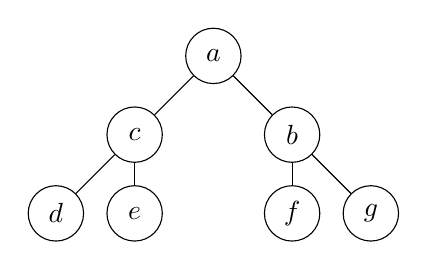
\begin{tikzpicture}
                    [scale=1, auto=left, every node/.style={minimum size=2em}]
                    \tikzset{edge/.style = {> = latex'}}
                    \node[circle,draw] (q1) at (0,0)    {$a$};
                    \node[circle,draw] (q2) at (1,-1)   {$b$};
                    \node[circle,draw] (q3) at (-1,-1)  {$c$};
                    \node[circle,draw] (q4) at (-2,-2)  {$d$};
                    \node[circle,draw] (q5) at (-1,-2)  {$e$};
                    \node[circle,draw] (q6) at (1,-2)   {$f$};
                    \node[circle,draw] (q7) at (2,-2)   {$g$};

                    \foreach \from/\to in {q1/q2,q1/q3,q2/q6,q2/q7,q3/q4,q3/q5}
                        \draw[edge] (\from) to (\to);
                \end{tikzpicture}
            }
         \end{center}
    \end{column}
    \end{columns}
\end{frame}

\begin{frame}[t]
    \frametitle{Teilbäume und Ordnung von Knoten}
    \only<1-2>{
        $T,T'$ gewurzelte Bäume.\\

        \begin{itemize}
            \setlength\itemsep{1.2em}
            \item Schreibe $T'\leq T$ wenn $T'$ Teilgraph von $T$.
            \pause
            \item Schreibe $T' \leq_{\color{red}{r}} T$ wenn $T' \leq T$ und $T,T'$ {\color{red}$r$-är}.\\[5pt]
        \end{itemize}
    }
    \only<3>{
        $v,v' \in V(T)$.\\
        Schreibe $v' \leq v$ genau dann, wenn der eindeutige Pfad von $root(T)$ zu $v$
        den Knoten $v'$ besucht. Hier $root(T) = a$:
    }
    \pause
    \begin{center}
        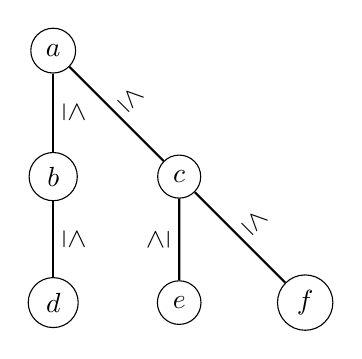
\begin{tikzpicture}
            [scale=0.8, auto=left]
            \tikzset{edge/.style = {> = latex'}}
            \node[circle,draw] (q1) at (0,4)  {$a$};
            \node[circle,draw] (q2) at (0,2)  {$b$};
            \node[circle,draw] (q3) at (2,2)  {$c$};
            \node[circle,draw] (q4) at (0,0)  {$d$};
            \node[circle,draw] (q5) at (2,0)  {$e$};
            \node[circle,draw] (q6) at (4,0)  {$f$};

        \only<3>{
            \draw (q1) [-,line width=.8pt] -- node[sloped,above] {$\leq$} (q2);
            \draw (q1) [-,line width=.8pt] -- node[sloped,above] {$\leq$} (q3);
            \draw (q2) [-,line width=.8pt] -- node[sloped,above] {$\leq$} (q4);
            \draw (q3) [-,line width=.8pt] -- node[sloped,above] {$\geq$} (q5);
            \draw (q3) [-,line width=.8pt] -- node[sloped,above] {$\leq$} (q6);
        }
        \end{tikzpicture}
    \end{center}
\end{frame}

\begin{frame}[t]
    \frametitle{Teilbäume und Ordnung von Knoten}
    Sei $root(T) \neq v \in V(T)$. Wir wollen $v$ und seine ''Nachfolger'' $w \in V(T)$ mit $v \leq w$
    aus $T$ inklusive Kanten ''ausschneiden''.

    \begin{center}
        \begin{tikzpicture}
            [scale=0.8, auto=left]
            \tikzset{edge/.style = {> = latex'}}

            \node[circle,draw] (q1) at (0,4)  {$a$};
            \node[circle,draw] (q2) at (0,2)  {$b$};
            \node[circle,draw] (q4) at (0,0)  {$d$};

            \draw (q1) [-,line width=.8pt] -- (q2);
            \draw (q2) [-,line width=.8pt] -- (q4);

            \only<1>{
                \node[circle,draw] (q5) at (2,0)  {$e$};
                \node[circle,draw] (q6) at (4,0)  {$f$};

                \draw (q3) [-,line width=.8pt] -- (q5);
                \draw (q3) [-,line width=.8pt] -- (q6);
            }

            \only<1-2>{
                \draw (q1) [-,line width=.8pt] -- (q3);
            }

            \only<1-3>{
                \node[circle,draw,fill=red] (q3) at (2,2)  {\textcolor{white}{$v$}};
            }

            \only<2-3>{
                \node[circle,draw,fill=red] (q5) at (2,0)  {\textcolor{white}{$w$}};
                \node[circle,draw,fill=red] (q6) at (4,0)  {\textcolor{white}{$w$}};

                \draw (q3) [-,line width=.8pt,color=red] -- node[sloped,above] {$\geq$} (q5);
                \draw (q3) [-,line width=.8pt,color=red] -- node[sloped,above] {$\leq$} (q6);
            }

            \only<3>{
                \node at (-1.6, 4) {$root(T) = $};
                \node at (3.8, 2) {$ = root(T')$};
                \draw (q1) [dashed,line width=.5pt] -- (q3);
            }

            \only<4>{
                \node at (-2,4) {$root(T \setminus v) = $};
                \node at (3,4) {};
            }
        \end{tikzpicture}
    \end{center}

    \only<3->{
        Definiere $T \setminus v := T \setminus T'$, wobei $T' \leq T$ der Teilbaum
        von $T$ mit Wurzel $v \in V(T) \setminus \{root(T)\}$ ist.\\
        Insbesondere ist $T \setminus v$ wieder ein gewurzelter Baum.
    }
\end{frame}

\begin{frame}
    \frametitle{Code als Baum}
    Sei $\mathcal{C}$ ein Code über dem Code-Alphabet $\{0,1,2\}$.\\
    $\mathcal{C}$ als Teilmenge von $V(T)$, wobei $T$:\\[30pt]
    \begin{center}
        \begin{forest}
            [$\varepsilon$
                [$0$
                    [$00$],
                    [$01$],
                    [$02$]
                ],
                [$1$
                    [$10$],
                    [$11$],
                    [$12$]
                ],
                [$2$
                    [$20$],
                    [$21$],
                    [$22$]
                ]
            ]
        \end{forest}\\
        \centerline{\LARGE\dots\ \,\quad\qquad\dots\ \,\quad\qquad\dots}
    \end{center}
\end{frame}

\begin{frame}[t]
    \frametitle{Code als Baum}

    \begin{itemize}
        \setlength\itemsep{1em}
        \item $h,r \in \mathbb{N}, A := [0,r-1]$ Code-Alphabet eines $r$-ären Codes $\mathcal{C}$
            mit max. Wortlänge $h$.
        \pause
        \item $W := \bigcup_{i \in [0,h]} A^i$ Menge aller Wörter über $A$ mit Länge $\leq h$.
        \pause
        \item Definiere gewurzelten $r$-ären Baum $\mathcal{T}_r^h$ der Höhe $h$ durch:
    \end{itemize}
    $$
        V(\mathcal{T}_r^h) := \{v_w \mid w \in W\}
    $$

    $$
        root(\mathcal{T}_r^h) := v_\varepsilon
    $$
    \pause
    $$
        E(\mathcal{T}_r^h) := \{(v_w,v_{w'}) \mid w,w' \in W, wx = w', x\in A\}
    $$
    \pause

    Inbesondere $\mathcal{T}_r^h$ eindeutig durch $r,h$ bestimmt.
\end{frame}

\begin{frame}[t]
    \frametitle{Bemerkungen zu $\mathcal{T}_r^h$}
    Betrachte $\mathcal{T}_3^2$:
    \begin{center}
        \only<1-2>{
        \Large
        \begin{forest}
            [$v_\varepsilon$
                [$v_0$
                    [$v_{00}$],
                    [$v_{01}$],
                    [$v_{02}$]
                ],
                [$v_1$
                    [$v_{10}$],
                    [$v_{11}$],
                    [$v_{12}$]
                ],
                [$v_2$
                    [$v_{20}$],
                    [$v_{21}$],
                    [$v_{22}$]
                ]
            ],
        \end{forest}\\
        }
        \only<3->{
        \Large
        \begin{forest}
            [\LARGE $v_{\color{red}\varepsilon}$
                [$v_0$
                    [$v_{00}$],
                    [$v_{01}$],
                    [$v_{02}$]
                ],
                [\LARGE $v_{\color{red}1}$, edge label={node [midway, sloped, above] {\color{blue}$\geq$}}
                    [\LARGE$v_{{\color{red}1}0}$, edge label={node [midway, sloped, above] {\color{blue}$\geq$}}],
                    [\LARGE$v_{{\color{red}1}1}$, edge label={node [midway, sloped, above] {\normalsize\color{blue}$\leq$}}],
                    [\LARGE$v_{{\color{red}1}2}$, edge label={node [midway, sloped, above] {\color{blue}$\leq$}}]
                ],
                [$v_2$
                    [$v_{20}$],
                    [$v_{21}$],
                    [$v_{22}$]
                ]
            ],
        \end{forest}\\
        }
    \end{center}
    \pause
    Wir haben:
    \begin{itemize}
        \setlength\itemsep{2em}
        \item Für $v_w \in V(\mathcal{T}_r^h)$ gilt $height(v_w) = |w|$.
        \pause
        \item Für $v_w, v_{w'} \in V(\mathcal{T}_r^h)$ gilt
            $v_w\ {\color{blue}\leq}\ v_{w'} \,\Longleftrightarrow\, w\ {\color{red}\sqsubseteq}\ w'$.
    \end{itemize}
\end{frame}

\section{Ungleichung von Kraft}
\begin{frame}
    \frametitle{Ungleichung von Kraft}
    Seien $q,r \in \mathbb{N}, l \in \mathbb{N}^q$. Dann existiert ein $r$-ärer sofort dekodierbarer Code $\mathcal{C}$
    mit Wortlängen $l$ genau dann, wenn
    $$
        \sum_{k=1}^{q} \frac{1}{r^{l_k}} \leq 1
    $$\\[20pt]
    \pause

    Annahmen:

    \begin{itemize}
        \setlength\itemsep{1em}
        \item Anzahl Code-Wörter $q > 1$
        \pause
        \item Wortlängen $l$ aufsteigend sortiert und $l_1 > 0$
        \pause
        \item Code-Alphabet von $\mathcal{C}$ ist $[0,r-1]$
    \end{itemize}
\end{frame}

\begin{frame}[t]
    \frametitle{Ungleichung von Kraft: Beweisidee ''$\,\Longrightarrow\,$''}
    Richtung ''$\sum_{k=1}^{q} \frac{1}{r^{l_k}} \leq 1 \,\Longrightarrow\,$ $\mathcal{C}$ existiert''.\\[10pt]
    \pause
    Nach [JJ00]: $\mathcal{C}$ sofort dekodierbar $\,\Longleftrightarrow\,$ $\mathcal{C}$ Präfixcode.\\
    \pause
    Am Beispiel
    $
    q=3,
    {\only<2-3>{\color{red}}r=2},
    l=(
    {\only<4>{\color{blue}}1},
    {\only<7>{\color{blue}}2},
    {\only<2-3>{\color{blue}}3})
    $.\only<10>{ $w_1=0,w_2=11,w_3=101$}
    \only<1-9>{
        Betrachte
        \only<1-6>{$\mathcal{T}_{\only<2-3>{\color{red}}2}^{\only<2-3>{\color{blue}}3}$}
        \only<7-8>{$\mathcal{T}_2^3 \setminus v_0$}
        \only<9>{$(\mathcal{T}_2^3 \setminus v_0) \setminus v_{11}$}:\\
        \only<5-9>{
            {\only<5>{\color{blue}}$w_1 = {\only<6>{\color{red}}0}$},
            \only<7-9>{
                {\only<7>{\color{blue}}$w_2 = {\only<8>{\color{red}}11}$},
                \only<9>{{\color{blue}$w_3 = 101$}}
            }
        }
    }
    \pause
    \strut\\[20pt]
    \begin{center}
        \only<3>{
        \begin{forest}
            [$v_\varepsilon$
                [$v_0$
                    [$v_{00}$
                        [$v_{000}$],
                        [$v_{001}$]
                    ],
                    [$v_{01}$
                        [$v_{010}$],
                        [$v_{011}$]
                    ]
                ],
                [$v_1$
                    [$v_{10}$
                        [$v_{100}$],
                        [$v_{101}$]
                    ],
                    [$v_{11}$
                        [$v_{110}$],
                        [$v_{111}$]
                    ]
                ]
            ]
        \end{forest}
        }
        \only<4>{
        \begin{forest}
            [$v_\varepsilon$
                [$v_0$,circle,draw,blue
                    [$v_{00}$
                        [$v_{000}$],
                        [$v_{001}$]
                    ],
                    [$v_{01}$
                        [$v_{010}$],
                        [$v_{011}$]
                    ]
                ],
                [$v_1$,circle,draw,blue
                    [$v_{10}$
                        [$v_{100}$],
                        [$v_{101}$]
                    ],
                    [$v_{11}$
                        [$v_{110}$],
                        [$v_{111}$]
                    ]
                ]
            ]
        \end{forest}
        }
        \only<5>{
        \begin{forest}
            [$v_\varepsilon$
                [$v_0$,circle,draw,blue
                    [$v_{00}$
                        [$v_{000}$],
                        [$v_{001}$]
                    ],
                    [$v_{01}$
                        [$v_{010}$],
                        [$v_{011}$]
                    ]
                ],
                [$v_1$
                    [$v_{10}$
                        [$v_{100}$],
                        [$v_{101}$]
                    ],
                    [$v_{11}$
                        [$v_{110}$],
                        [$v_{111}$]
                    ]
                ]
            ]
        \end{forest}
        }
        \only<6>{
            \begin{forest}
            [$v_\varepsilon$
                [$v_{\color{red}0}$
                    [$v_{{\color{red}0}0}$
                        [$v_{{\color{red}0}00}$],
                        [$v_{{\color{red}0}01}$]
                    ],
                    [$v_{{\color{red}0}1}$
                        [$v_{{\color{red}0}10}$],
                        [$v_{{\color{red}0}11}$]
                    ]
                ],
                [$v_1$
                    [$v_{10}$
                        [$v_{100}$],
                        [$v_{101}$]
                    ],
                    [$v_{11}$
                        [$v_{110}$],
                        [$v_{111}$]
                    ]
                ]
            ]
        \end{forest}
        }
        \only<7>{
            \begin{forest}
            [$v_\varepsilon$
                [$v_1$
                    [$v_{10}$
                        [$v_{100}$],
                        [$v_{101}$]
                    ],
                    [$v_{11}$,circle,draw,blue
                        [$v_{110}$],
                        [$v_{111}$]
                    ]
                ]
            ]
        \end{forest}
        }
        \only<8>{
            \begin{forest}
            [$v_\varepsilon$
                [$v_1$
                    [$v_{10}$
                        [$v_{100}$],
                        [$v_{101}$]
                    ],
                    [$v_{\color{red}11}$
                        [$v_{{\color{red}11}0}$],
                        [$v_{{\color{red}11}1}$]
                    ]
                ]
            ]
            \end{forest}
        }
        \only<9>{
            \begin{forest}
            [$v_\varepsilon$
                [$v_1$
                    [$v_{10}$
                        [$v_{100}$],
                        [$v_{101}$,circle,draw,blue]
                    ]
                ]
            ]
            \end{forest}
        }
        \only<10->{
            \begin{itemize}
                \setlength\itemsep{1.5em}
                \item $q = 3$ Wörter über Alphabet $[0,r-1] = [0,1] = \{0,1\}$.
                \item Wortlängen $|w_1| = l_1, |w_2| = l_2, |w_3| = l_3$ eingehalten.
                \item Präfixcode $\mathcal{C} = \{w_1,w_2,w_3\} = \{0,11,101\}$ konstruiert.
            \end{itemize}
        }
    \end{center}
\end{frame}

\begin{frame}[t]
    \frametitle{Ungleichung von Kraft: ''$\,\Longrightarrow\,$''}

    \begin{columns}
    \begin{column}{0.5\textwidth}
        \only<1-3>{
            Sei also $i = 1$. Wähle Knoten $v_w$ der Höhe $l_1 > 0$ beliebig und setze $w_i = w_1 := w$.\\[10pt]\pause
            Setze $h := l_q$ (max. Wortlänge) und
            $\mathcal{T}_0 := \mathcal{T}_r^h,\ \mathcal{T}_1 := \mathcal{T}_r^h \setminus v_{w_1}$.\\[10pt]
        }\pause
        $\mathcal{T}_1$ hat dann noch
        $r^h - r^{h -l_1}$ Blätter.\\
        \only<4->{
            Weiter gilt:
            $$
                r^h - r^{h - l_1} = r^h\left(1 - \sum_{k=1}^{1} \frac{1}{r^{l_k}}\right)
            $$
            \only<5->{
                $$
                    > r^h\left(1 - \sum_{k=1}^{q} \frac{1}{r^{l_k}}\right) \only<6>{\geq 0}
                $$
            }
        }
    \end{column}

    \begin{column}{0.5\textwidth}
        \onslide
            \only<1>{
            \quad$\mathcal{T}_r^h$:\\
            \begin{center}
                \begin{forest}
                    [$v_\varepsilon$
                        [$v_0$,
                            [\dots]
                        ],
                        [$v_1$
                            [\dots
                                [$v_w$,color=red,
                                    [$v_{w0}$
                                        [\dots]
                                    ],
                                    [$v_{w1}$
                                        [\dots]
                                    ],
                                    [\dots]
                                ],
                            ],
                            [\dots]
                        ],
                        [\dots]
                    ]
                \end{forest}
            \end{center}
            }
            \only<2>{
            \quad$\mathcal{T}_r^h$:\\
            \begin{center}
                \begin{forest}
                    [$v_\varepsilon$
                        [$v_0$,
                            [\dots]
                        ],
                        [$v_1$
                            [\dots
                                [$v_w$,color=red,tikz={\node [draw,red,fit=()(!1)(!11)(!2)(!3)] {};}
                                    [$v_{w0}$
                                        [\dots]
                                    ],
                                    [$v_{w1}$
                                        [\dots]
                                    ],
                                    [\dots]
                                ],
                            ],
                            [\dots]
                        ],
                        [\dots]
                    ]
                \end{forest}
            \end{center}
            }
            \only<3->{
            \begin{center}
                \begin{tikzpicture}
                    \node[color=red] at (0.5,-3) {$v_{w_1}$};
                    \node at (0,-1.5) {$\mathcal{T}_1$};

                    \draw (0,0) node[above]{$v_\varepsilon$}
                        -- (-2.5,-4)
                        -- (-.5,-4)
                        -- (0.5,-2.4)
                        -- (1.5,-4)
                        -- (2.5,-4)
                        -- cycle;

                    \draw[|-|] (-.5,-4.5) -- node[below] {$r^{h-l_1}$} (1.5,-4.5);

                    \draw[|-|] (-2.5,-5.4) -- node[below] {$r^h$} (2.5,-5.4);
                \end{tikzpicture}
            \end{center}
            }
    \end{column}
    \end{columns}
\end{frame}

\begin{frame}[t]
    \frametitle{Ungleichung von Kraft: ''$\,\Longrightarrow\,$''}
    Nun $i \in [1,q-1]$ sodass $\{w_j \mid j \in [1,i]\}$ ein Präfix-Code
    mit $|w_j| = l_j$ ist, und $\mathcal{T}_i$ noch mindestens 1 Blatt $v_x$ hat.\\[10pt]\pause

    \begin{columns}
    \begin{column}{0.77\textwidth}
        \begin{itemize}
            \item $\mathcal{T}_i$ zusammenhängend\\[10pt]
            \item also ex. $v_w \in V(\mathcal{T}_i)$ mit $height(v_w) = l_{i+1} \leq h$\\[10pt]
            \item Setze $w_{i+1} := w$.
        \end{itemize}
    \end{column}
    \begin{column}{0.23\textwidth}\onslide
        \begin{center}
            \only<1>{
                \begin{forest}
                    [$v_\varepsilon$
                        [\vdots
                            [$v_{x}$]
                        ]
                    ]
                \end{forest}
            }
            \only<2->{
                \begin{forest}
                    [$v_\varepsilon$
                        [\vdots
                            [$v_{w_{i+1}}$,color=blue
                                [\vdots
                                    [$v_x$]
                                ]
                            ]
                        ]
                    ]
                \end{forest}
            }
        \end{center}
    \end{column}
    \end{columns}
\end{frame}

\begin{frame}[t]
    \frametitle{Ungleichung von Kraft: ''$\,\Longrightarrow\,$''}
    \only<1>{Sei $j \in [1,i]$. Wir haben bereits alle Knoten $v_w \geq v_{w_j}$ im Schritt
    $\mathcal{T}_j := \mathcal{T}_{j-1} \setminus v_{w_j}$ gelöscht. Da wir $v_{w_{i+1}}$
    aus $\mathcal{T}_i$ gewählt haben, kann also \textbf{nicht} $v_{w_j} \leq v_{w_{i+1}}$ gelten.} \pause
    \only<2->{
        Folglich haben wir auch $w_j \not\sqsubseteq w_{i+1}$ für $j \in [1,i]$. $\mathcal{C}$ bleibt also
        durch Wahl von $w_{i+1}$ ein Präfix-Code ($l_j \leq l_{i+1}$, also $w_{i+1} \not\sqsubseteq w_j$).
    }
    \pause
    \only<3->{
        \\[10pt]
        Wenn $i+1 = q$, so haben wir $q$ Wörter gewählt und sind fertig.\pause\\[10pt]
        Falls hingegen $i+1 < q$, so definiere $\mathcal{T}_{i+1} := \mathcal{T}_i \setminus v_{w_{i+1}}$.\\
        Dann hat $\mathcal{T}_{i+1}$ immernoch mindestens 1 Blatt, denn:
        \only<4>{
        $$
            \mathcal{T}_i\ \text{hat nach Konstruktion}\quad
            r^h - \sum_{k=1}^{i} r^{h-l_k}
            \quad\text{Blätter}
        $$
        }
        \pause
        \only<5->{
            \\
            $\mathcal{T}_{i+1}$ hat nach Konstruktion also:
            $$
                r^h - \sum_{k=1}^{i+1} r^{h-l_k}
                \pause
                > r^h - \sum_{k=1}^{q} r^{h-l_k}
                \pause
                = r^h \left(1 - \sum_{k=1}^{q} \frac{1}{r^{l_k}}\right)
                \pause
                \geq 0
            $$
            Blätter.\\[5pt]
            Somit Präfixcode $\mathcal{C}$ nach dieser Methode konstruierbar.\\
            Dieser ist nach [JJ00] auch sofort dekodierbar.
        }
    }

    \only<1-2>{
    \begin{center}\onslide
        \begin{tikzpicture}
            \node[color=red] at (2,-4) {$v_{w_1}$};
            \node[color=red] at (-4.5,-5) {$v_{w_j}$};
            \node[color=red] at (-2.5,-5.2) {$v_{w_k}$};
            \node[color=blue] at (-0.2,-5) {$v_{w_{i+1}}$};
            \node at (-1,-5.8) {$v_x$};
            \node at (0,-1.5) {$\mathcal{T}_i$};

            \draw (0,0)
                -- (-4.5,-4.5)
                -- (-3.5,-5.5)
                -- (-3.25,-5.5)
                -- (-2.5,-4.75)
                -- (-1.75,-5.5)
                -- (0,-5.5)
                -- (2,-3.5)
                -- (4,-5.5)
                -- (5.5,-5.5)
                -- cycle;

            \draw[dashed] (0,0)
                -- (0,-0.15)
                -- (-1,-1.15)
                -- (0,-2)
                -- (-1.5,-3.5)
                -- (-1,-4)
                -- (-1.25,-4.25)
                -- (-0.5,-5)
                -- (-1,-5.5);
        \end{tikzpicture}
    \end{center}
    }
\end{frame}

\begin{frame}[t]
    \frametitle{Ungleichung von Kraft: ''$\,\Longleftarrow\,$''}
    \only<1-2>{
        Nun zeigen wir, dass wenn $\mathcal{C}$ sofort dekodierbar, also ein Präfix-Code ist, auch
        die Ungleichung gelten muss. \pause\\
        Betrachte für $i \in [1,q]$ die Menge der Blätter unter $v_{w_i}$:
    }
    \only<2->{
        $$
            {\color{red}L_i} := \{v \in V(\mathcal{T}_r^h) \mid v_{w_i} \leq v \land height(v) = h\}
        $$
        \begin{center}\onslide
            \begin{tikzpicture}
                \node at (0,-1) {$\mathcal{T}_r^h$};
                \node at (.5, -2.3) {$v_{w_i}$};
                \node[color=red] at (.5, -4.3) {$L_i$};

                \draw (0,0)
                    -- (-4,-4)
                    -- (4,-4)
                    -- cycle;

                \draw[dashed] (-1,-4) -- (.5, -2.5) -- (2,-4);

                \draw[line width = 2pt, color=red] (-1,-4) -- (2,-4);
            \end{tikzpicture}
        \end{center}
    }
\end{frame}

\begin{frame}[t]
    \frametitle{Ungleichung von Kraft: ''$\,\Longleftarrow\,$''}
    Für $i,j \in [1,q]$ mit $i \neq j$ ist $L_i \cap L_j = \varnothing$\only<1-5>{, denn:} \pause
    \only<2-5>{
        \\[10pt]
        Sei o.E. $i < j, v_w \in L_i \cap L_j$, also $v_w$ gleichzeitig Blatt unter $v_{w_i},v_{w_j}$.\\
        \pause
        Dann gilt:
        $$
            v_{w_i} \leq v_w \land v_{w_j} \leq v_w
            \pause \,\Longrightarrow\,
            w_i \sqsubseteq w \land w_j \sqsubseteq w
            \pause \,\Longrightarrow\,
            w_i \sqsubseteq w_j
        $$
        Widerpruch, denn $w_i, w_j \in \mathcal{C}$ und $\mathcal{C}$ ist Präfix-Code!
        \pause
    }
    \only<6->{
        \\[10pt]
        Weiter hat $\mathcal{T}_r^h$ nur $r^h$ Blätter, und $|L_i| = r^{h-l_i}$.
        \only<9->{
            \\[10pt]
            Damit haben wir nun:
            $$
                r^h \geq \left| \bigcup_{i \in [1,q]} L_i \right|
            \only<10->{
                = \sum_{i=1}^{q} |L_i|
            }\only<11->{
                = \sum_{i=1}^{q} r^{h-l_i}
                = r^h\sum_{i=1}^{q} \frac{1}{r^{l_i}}
            }
            $$
            \only<12->{
                $$
                    \,\Longleftrightarrow\, \sum_{i=1}^{q} \frac{1}{r^{l_i}} \leq 1
                $$
                Dies war zu zeigen. \hfill $\square$
            }
        }
        \only<6-8>{
            \\[30pt]
            \begin{center}\onslide
                \begin{tikzpicture}
                    \node at (0,-1) {$\mathcal{T}_r^h$};
                    \node at (.5, -2.3) {$v_{w_i}$};
                    \node[color=red] at (.5, -4.3) {$L_i$};

                    \draw (0,0)
                        -- (-4,-4)
                        -- (4,-4)
                        -- cycle;

                    \draw[dashed] (-1,-4) -- (.5, -2.5) -- (2,-4);

                    \draw[line width = 2pt, color=red] (-1,-4) -- (2,-4);

                    \only<6-8>{
                        \draw[dotted, line width = .8pt] (-5.5, -2.5) -- (.5, -2.5);
                        \draw[dotted, line width = .8pt] (-5.5, 0) -- (0, 0);
                        \draw[|-|, line width = .8pt] (-5.5,-2.5) --
                            node[right] {$height(v_{w_i}) = |w_i| = l_i$} (-5.5, 0);
                    }
                    \only<7-8>{
                        \draw[dotted, line width = .8pt] (-5.5, -2.5) -- (.5, -2.5);
                        \draw[|-|, line width = .8pt] (-5.5,-4) -- node[right] {$h-l_i$} (-5.5, -2.5);
                    }
                    \only<8>{
                        \draw[|-|, line width = .8pt] (-1,-4.6) -- node[below] {$r^{h-l_i}$} (2,-4.6);
                    }
                \end{tikzpicture}
            \end{center}
        }
    }
\end{frame}

\begin{frame}[t]
    \frametitle{Review of Kraft or smth.}
    Wir haben also gezeigt:\\[5pt]
    Seien $q,r \in \mathbb{N}, l \in \mathbb{N}^q$. Dann existiert ein $r$-ärer sofort dekodierbarer Code $\mathcal{C}$
    mit Wortlängen $l$ genau dann, wenn
    $$
        \sum_{k=1}^{q} \frac{1}{r^{l_k}} \leq 1
    $$
    \begin{itemize}
        \item Wissen nun, wie so ein Code erstellt werden kann
    \end{itemize}
\end{frame}


\section{Ungleichung von McMillan}

\begin{frame}[t]
    \frametitle{Ungleichung von McMillan}
    Seien $q,r \in \mathbb{N}, l \in \mathbb{N}^q$. Dann existiert ein $r$-ärer eindeutig dekodierbarer Code $\mathcal{C}$
    mit Wortlängen $l$ genau dann, wenn
    \begin{equation}
        K := \sum_{k=1}^{q} \frac{1}{r^{l_k}} \leq 1
    \end{equation}\\[20pt]
    \pause

    Richtung ''$(1) \,\Longrightarrow\, \mathcal{C}$ existiert'' folgt sofort mit Kraft.\\
\end{frame}

\begin{frame}[t]
    \frametitle{Ungleichung von McMillan: Beweisidee}
    \begin{itemize}
        \setlength\itemsep{1em}
        \item Zu zeigen: $K = \sum_{k=1}^{q} \frac{1}{r^{l_k}} \leq 1$
        \pause
        \item Betrachte $K^n$ für beliebiges $n \in \mathbb{N}$.
        \pause
        \item $K^n$ als Summe abhängig von Wahl von $n$ Wortlängen aus $l$.
        \pause
        \item Fasse Auswahlen (Indextupel) mit selbem Summand zusammen
            und summiere über möglichen Wertebereich
        \pause
        \item Nun finde aus Form von $K^n$ konstante obere Schranke
        \pause
        \item Dann muss $K \leq 1$, da sonst $K^n$ für geeignetes $n$ größer
            als jede Konstante
    \end{itemize}
\end{frame}

\begin{frame}[t]
    \frametitle{Ungleichung von McMillan: ''$\,\Longleftarrow\,$''}
        Wir müssen also zeigen, dass $K \leq 1$, wobei
        $$
            K = \sum_{k=1}^{q} \frac{1}{r^{l_k}}
        $$
        \pause
        Sei $n \in \mathbb{N}$. Wir betrachten:
        $$
            K^n = \left(\sum_{k=1}^{q} \frac{1}{r^{l_k}}\right)^n
            \pause
            = \sum_{i \in [1,q]^n} \prod_{k=1}^{n} \frac{1}{r^{l_{i_k}}}
            \pause
            = \sum_{i\in [1,q]^n} r^{-\sum_{k=1}^{n} l_{i_k}}
        $$\pause

        Werden Summe über Auswahl an Wortlängen noch oft brauchen, definiere:
        $$
            \mathcal{S}: [1,q]^n \to \mathbb{N},\ i \mapsto \sum_{k=1}^{n} l_{i_k}
        $$
\end{frame}

\begin{frame}[t]
    \frametitle{Ungleichung von McMillan: Beispiel}
        Anzahl Codewörter $q = 3$. Wortlängen $l = (1,3,5)$. $n = 2$.
        \only<1-2>{
            $$
                [1,q]^n = \{(1,1), (1,2), (1,3), (2,1), (2,2), (2,3), (3,1), (3,2), (3,3)\}
            $$$$
                i = (3,1) \in [1,q]^n \,\Longrightarrow\, \mathcal{S}(i) = \sum_{k=1}^{n} l_{i_k}
                = l_{i_1} + l_{i_2} = l_3 + l_1 = 5 + 1 \only<2>{= \color{red} \text{\LARGE 6}}
            $$$$
                i = (2,3) \in [1,q]^n \,\Longrightarrow\, \mathcal{S}(i) = \sum_{k=1}^{n} l_{i_k}
                = l_2 + l_3 = 3 + 5
            $$$$
                i = (2,2) \in [1,q]^n \,\Longrightarrow\, \mathcal{S}(i) = \sum_{k=1}^{n} l_{i_k}
                = l_2 + l_2 = 3 + 3 \only<2>{= \color{red} \text{\LARGE 6}}
            $$
            \only<2>{Also auch selber Wert bei unterschiedlichen Indextupeln.}
        }
        \only<3->{
            \only<3-4>{
                \\[5pt]
                \begin{itemize}
                    \item Summe minimal $3$, maximal $15$.
                    \item Fasse Indextupel mit gleicher Summe $j \in [3,15]$ zusammen
                \end{itemize}
                $$
                    N_{\only<3>{\color{red}}6} := \mathcal{S}^{-1}(\{{\only<3>{\color{red}}6}\}) = 
                        \{i \in [1,3]^2 \mid \mathcal{S}(i) = {\only<3>{\color{red}}6}\}
                    = \{\underbrace{(1,3)}_{l_1+l_3 = {\only<3>{\color{red}}6}},
                        \overbrace{(3,1)}^{l_3+l_1 = {\only<3>{\color{red}}6}},
                        \underbrace{(2,2)}_{l_2+l_2 = {\only<3>{\color{red}}6}}\}
                $$
                \only<4>{
                    $$
                        N_{\color{red}j} :=
                        \mathcal{S}^{-1}({\color{red}j})
                        = \{i \in [1,q]^n \mid \mathcal{S}(i) = \sum_{k=1}^{n} l_{i_k} = {\color{red}j}\}
                    $$
                }
            }
            \only<5->{\\
                \begin{itemize}
                    \setlength\itemsep{1em}
                    \item Betrachte Alphabet $[0,1], \mathcal{C}
                        = \{\underbrace{0}_{w_1},
                            \underbrace{100}_{w_2},
                            \underbrace{11111}_{w_3}\}$
                \only<6->{
                    \item Zu $i \in [1,q]^n$ eindeutige Code-Sequenz
                        $\mathcal{W}(i) = w_{i_1}w_{i_2}\cdots w_{i_n}$.
                }\\[15pt]
                \end{itemize}
                \only<7->{
                    $$
                        \mathcal{W}(N_6)
                        = \{\mathcal{W}(t) \mid t \in N_6\}
                        = \{\mathcal{W}(t) \mid t \in \{(1,3),(3,1),(2,2)\}\}
                    $$
                    $$
                        = \{w_1w_3, w_3w_1, w_2w_2\}
                        = \{011111,111110,100100\}
                    $$
                    \only<8->{\\[10pt]
                        Da $N_6$ gerade die Indextupel Wortlängensumme $6$:
                        $$
                            \forall i \in N_6: |\mathcal{W}(i)| = 6
                            \qquad\text{und}\qquad
                            \mathcal{W}(N_6) \subseteq \{0,1\}^6
                        $$
                    }
                }
            }
        }
\end{frame}

\begin{frame}[t]
    \frametitle{Ungleichung von McMillan: ''$\,\Longleftarrow\,$''}
    Kürzeste Wortlänge $\displaystyle m := \min_{k \in [1,q]} l_k$,
    längste $\displaystyle M := \max_{k \in [1,q]} l_k$
    \pause
    \\Damit gilt auch
    $$
        n\cdot m \leq \mathcal{S}(i) = \sum_{k=1}^{n} l_{i_k} \leq n\cdot M
    $$
    für alle Indextupel $i \in [1,q]^n$.
    \pause
    Definiere für $j \in [nm, nM]$:
    $$
        N_j := \mathcal{S}^{-1}(j) = \{i \in [1,q]^n \mid \mathcal{S}(i) = \sum_{k=1}^{n} l_{i_k} = j\}
    $$
    \pause
    $$
        \mathcal{W} : [1,q]^n \to [0,r-1]^{*},\ i \mapsto w_{i_1}w_{i_2}\cdots w_{i_n}
    $$
    \pause\\
    $\mathcal{C}$ eindeutig dekodierbar $\,\Longrightarrow\,$ $\mathcal{W}$ injektiv, da
    $i \in [1,q]^n$ die eindeutige Kombination von Codewörtern aus $\mathcal{C}$ für $\mathcal{W}(i)$.
\end{frame}

\begin{frame}[t]
    \frametitle{Ungleichung von McMillan: ''$\,\Longleftarrow\,$''}
    $j \in [nm,nM]$ zwischen min / max Wortlängensumme.
    $$
        N_j := \mathcal{S}^{-1}(j),\quad
        \mathcal{W} : [1,q]^n \to [0,r-1]^{*},\ i \mapsto w_{i_1}w_{i_2}\cdots w_{i_n}
    $$
    \begin{itemize}
        \setlength\itemsep{1em}
        \item $\mathcal{W}$ injektiv $\,\Longrightarrow\, |N_j| = |\mathcal{W}(N_j)|$
        \pause
        \item $|\mathcal{W}(i)| = j$ für $i \in N_j$ nach Konstruktion
        \pause
        \item $\mathcal{W}(N_j) \subseteq [0,r-1]^j \,\Longrightarrow\, |\mathcal{W}(N_j)| \leq |[0,r-1]^j|$
        \pause
        \item $|N_j| \leq r^j$
    \end{itemize}
\end{frame}

\begin{frame}[t]
    \frametitle{Ungleichung von McMillan: ''$\,\Longleftarrow\,$''}
        \only<1>{
            Recap:
        }
        $$
            K := \sum_{i=1}^{q} \frac{1}{r^{l_i}}
        $$
        $$
            K^n = \sum_{i\in [1,q]^n} r^{-\sum_{k=1}^{n} l_{i_k}} = \sum_{i\in [1,q]^n} r^{-\mathcal{S}(i)}
        $$
        \pause
        \begin{itemize}
            \setlength\itemsep{1em}
            \item {\only<4>{\color{red}} $|N_j| \leq r^j$} Anzahl der $i \in [1,q]^n$ mit gleichem $\mathcal{S}(i)$.
            \pause
            \item Fasse zusammen via $N_j$, summiere über $[nm,nM]$
        \end{itemize}
        \strut\\
        $$
            K^n = \sum_{j = nm}^{nM} |N_j|r^{-j} = \sum_{j = nm}^{nM} \frac{|N_j|}{r^j}
            \only<4>{
                \quad{\color{red}\leq}\quad \sum_{j = nm}^{nM} 1
                = (M-m)n + 1
            }
        $$
\end{frame}

\begin{frame}[t]
    \frametitle{Ungleichung von McMillan: ''$\,\Longleftarrow\,$''}
    $$
        K := \sum_{i=1}^{q} \frac{1}{r^{l_i}},\quad K^n \leq (M-m)n + 1
        \only<2->{\,\Longrightarrow\, \frac{K^n}{n} \leq (M-m) + 1}
    $$
    \only<2->{
        \begin{itemize}
            \setlength\itemsep{1em}
            \item Code $\mathcal{C}$ gegeben; $q = |\mathcal{C}|$, Alphabetgröße $r$, Wortlängen $l$ fix.
            \item Damit auch $m,M,K$ fix.
            \pause
            \item $n \in \mathbb{N}$ beliebig; Ungleichung muss für alle $n \in \mathbb{N}$ gelten.
            \pause
            \item Nach Analysis bekannt: nur möglich für $K \leq 1$.
        \end{itemize}
        $$
            \,\Longrightarrow\, \sum_{i=1}^{q} \frac{1}{r^{l_i}} = K \leq 1
        $$
        \strut\hfill$\square$
    }
\end{frame}

\begin{frame}
    \frametitle{Review of McMillan or smth.}

    [...]
\end{frame}

\end{document}
